\documentclass[openany, 11pt]{memoir}
\usepackage[utf8]{inputenc}
\usepackage[T1]{fontenc}
\usepackage[english, french]{babel}

%%% Utility packages
% Lists
\usepackage{titletoc}
% Links
\usepackage{hyperref}
\hypersetup{
	colorlinks,
	linkcolor = blue!30!black,
	citecolor = blue!30!black,
	urlcolor = purple!40!black
}
\usepackage[colorinlistoftodos]{todonotes}
\presetkeys{todonotes}{inline, color=blue!40!red!20}{}
% Code
\usepackage{listings}
\lstset{
	literate={é}{{\'e}}1,
	basicstyle=\ttfamily,
	tabsize=4
}
% Bibliography
\usepackage{tocbibind}
\bibliographystyle{plain}
% Glossary
\usepackage[toc, automake]{glossaries}
% Custom commands
\newcommand{\acronymdesc}[4]{
	\newacronym[type=#1,description={#3~: #4}]{#2}{#2}{#3}
}

\newglossary[ad]{admin}{adm}{ado}{Glossaire administratif}
\newglossary[tc]{tech}{tch}{tco}{Glossaire technique}

% ADMINISTRATIF
\acronymdesc{admin}{DGFiP}
	{Di\-rec\-tion Gé\-né\-rale des Fi\-nan\-ces Pu\-bli\-ques}
	{Service public de l'État rattaché au ministère des finances, chargé des missions de gestion publique et de fiscalité}

\acronymdesc{admin}{DGCP}
	{Di\-rec\-tion Gé\-né\-rale des Comptes Pu\-blics (DGCP)}
	{Aussi appelée <<trésor public>>, ancienne administration chargée de la gestion des comptes de l'État et du recouvrement des impôts}
	
\acronymdesc{admin}{DGI}
	{Di\-rec\-tion Gé\-né\-rale des Impôts}
	{Ancienne administration chargée de la liquidation des impôts}
	
\acronymdesc{admin}{SI}
	{Ser\-vice des sys\-tèmes d'In\-for\-ma\-tion}
	{Service support de la \gls{DGFiP} chargé de la gestion informatique et du développement d'applications}
	
\acronymdesc{admin}{DPN}
	{Dir\-ec\-tion des pro\-jets nu\-mé\-ri\-ques}
	{Direction au sein du \gls{SI} regroupant les différents bureaux en charge de la direction et de la réalisation de projets dans le numérique}

\acronymdesc{admin}{BSI-3}
	{Bu\-reau du SI des pro\-fes\-sion\-nels}
	{Bureau dépendant de la \gls{DPN}, chargé}

% TECHNIQUE
\acronymdesc{tech}{TAL}
	{trai\-te\-ment au\-to\-ma\-tique du lan\-gage}
	{Ensemble de méthodes visant à analyser et traiter le langage naturel}

\newglossaryentry{log}{
    name={log},
	type=tech,
    description={De l'anglais log (journal), sortie d'une application (souvent un fichier) représentant le chemin d'exécution d'une application}
}

\newglossaryentry{ml}{
    name={ap\-pren\-tis\-sage au\-to\-ma\-tique},
	type=tech,
    description={Ou \textit{machine learning} en anglais, ensemble de méthodes visant a développer des algorithmes généraux basés sur l'apprentissage de données, s'opposant a un algorithme explicite classique}
}

\newglossaryentry{deep}{
    name={ap\-pren\-tis\-sage pro\-fond},
	type=tech,
    description={Branche de l'\gls{ml} se basant sur des réseaux de neurones artificiels, comportant plusieurs couches de traitement de données permettant d'extraire des caractéristiques complexes}
}
\makeglossaries

%%% Display packages
\usepackage{graphicx}
\usepackage{fullpage}
\usepackage{xcolor}
% Fonts
\usepackage{helvet}
\usepackage{inconsolata}
\renewcommand{\familydefault}{\sfdefault}
\usepackage{fontawesome}
% Header
\usepackage{fancyhdr}
\setlength{\headheight}{16pt}
\setlength{\headsep}{10pt}
\lhead{\textit{\leftmark}}
\rhead{}
\fancyfoot[C]{\textsf{\thepage}}
% Lists
\usepackage[shortlabels]{enumitem}
\setlist[itemize,1]{label=\textbullet}
\setlist[itemize,2]{label=--}
% Spacing
\linespread{1.2}

%%% Custom commands
% Unnumbered in toc
\newcommand\chapters[1]{
	\chapter*{#1}
	\addcontentsline{toc}{chapter}{#1}
}

\newcommand\link[2]{
	\href{#1}{#2 {\small\faExternalLink}}
}

% Easily include image in annexes
\newcommand\anneximage[3]{
	\begin{figure}
		\centering
		 \includegraphics[angle=#2,height=0.93\textheight,width=\textwidth,keepaspectratio]{images/#1.png}
		\caption{#3}
		\label{#1}
	\end{figure}
}

\newenvironment{centerall}
    {\begin{center}\vspace*{\fill}}
    {\vspace*{\fill}\end{center}}

% DOCUMENT
\begin{document}
\frontmatter
\pagenumbering{gobble}

% Header
\begin{minipage}{0.5\textwidth}
	\Large
	Mémoire de PFE
	
	\vspace{10pt}
	Formation FIL
	
	\vspace{10pt}
	IMT Atlantique
\end{minipage}
\begin{minipage}{0.45\textwidth} % Deco graphics
	
\includegraphics[width=\textwidth]{images/header.png}
\end{minipage}

% Title
\begin{minipage}{\textwidth}
    \centering \LARGE
    \vspace{20pt}
    \textbf{Amélioration des performances de détection automatique d'anomalies dans des logs applicatifs}
	
    \vspace{5pt}
	Oscar Gloaguen
	
	\vspace{60pt}
    Direction Générale des Finances Publiques
\end{minipage}

% Logos
\vfill

\includegraphics[width=\textwidth]{images/logos.png}

\newpage
\pagenumbering{roman}
\tableofcontents
\startlist[main]{lof}

\newpage
\chapters{Remerciements}
Je souhaite remercier la Direction Générale des Finances Publiques et tout particulièrement Olivier Blanc, pour m'avoir permis d'effectuer mon alternance dans cette équipe et pour m'avoir accompagné tout au long jusqu'au PFE.

\bigskip
Je tiens a remercier personnellement Robin Gries, qui a su être un vrai coéquipier tout au long de ce projet malgré sa complexité.

\bigskip
Je voudrais aussi remercier IMT Atlantique ainsi que ses professeurs, et surtout mon tuteur pédagogique Thomas Ledoux qui s'est mis a ma disposition pour le PFE.

\newpage
\begin{abstract}
\addcontentsline{toc}{chapter}{Résumé}
Les \glspl{log} sont une source importante de données détaillant le fonctionnement interne d'une application, mais ne sont pourtant que rarement utilisés a leur plein potentiel. Dans ce mémoire, je vais détailler le processus d'évolution d'un outil d'\gls{ml} qui utilise les \glspl{log} pour détecter et même tenter de prévoir des anomalies logicielles. Le projet s'apparentant plus a un projet de recherche, la démarche scientifique sera détaillée, ainsi que les caractéristiques techniques et le déroulement de l'implémentation. L'organisation du projet avec un stagiaire et moi-même sera développée, ainsi que ses impacts humains et économiques.
\end{abstract}

{\selectlanguage{english} 
\begin{abstract}
\Glspl{log} are an important source of data when it comes to the internal workings of software, but they are rarely used to their full potential. In this memoir, I will explain the evolution of a machine learning tool which uses \glspl{log} to detect and even attempt to predict software anomalies. The project being similar to a research project, the scientific protocol will be detailed, as well as the technical characteristics and the course of the implementation. Project management with an intern and myself will be developed, as well as the human and economic impacts of the project.
\end{abstract}}

\paragraph{Mots-clés}
\gls{TAL}, apprentissage automatique, apprentissage profond, analyse de logs applicatifs

% Main content
\mainmatter
\pagestyle{fancy}
\glsresetall
\chapters{Introduction}
\todo{1-2 pages}

Le projet \texttt{analyse-logs} a été développé par deux précédents apprentis de la \gls{DGFiP}, Rémi puis Léa. Cependant, les performances des algorithmes implémentés n'étant pas satisfaisantes, c'est ici que nait le sujet de ce PFE. Ce mémoire détaille le processus d'évolution de ce projet dans l'objectif d'amélioration des performances.

\bigskip
J'ai travaillé sur cette problématique en binôme avec Robin, un stagiaire en dernière année de master. Ce document touchera aussi sur l'organisation du sujet entre nous ainsi que les bénéfices et difficultés a travailler en équipe.

\bigskip
Ce sujet de PFE s'intègre dans la stratégie d'innovation du SI de la \gls{DGFiP}. L'objectif est de montrer l'efficacité de ces outils, pour mettre en valeur l'innovation et pousser leur utilisation au sein des bureaux. Dans ce cadre, une structure proche de celle d'un projet de recherche a été suivie. Pour cela, nous avons d'abord composé et étudié un état de l'art des algorithmes de détection d'anomalies existants. Ils utilisent pour la plupart des méthodes d'\gls{ml}, avec des algorithmes classiques ou de l'\gls{deep}.

\newpage
\chapter{La DGFiP, administration en évolution constante}
\label{dgfip}
La \gls{DGFiP} est une administration française née de la fusion de la Direction \gls{DGI} et de la \gls{DGCP} en 2008. Elle hérite alors des missions des deux entités, en faisant un service public très étendu, en charge notamment de la collecte des impôts et taxes et de la législation fiscale. 

Cette administration possède une hiérarchie forte séparée en 8 services, qui définit leur domaine de travail, ainsi que différentes directions (voir organigramme \ref{orga} en annexes). Une majorité des services sont des services métiers, directement en lien avec les missions de la \gls{DGFiP}, mais 3 de ces services sont des services support, ou \glspl{transverse}. Ces derniers sont le service des Ressources Humaines, le service de Stratégie, Pilotage et Budget, et le \gls{SI}. Malgré une interaction indirecte avec le domaine métier des dinances publiques, ils répondent aux besoins de la \gls{DGFiP} en permettant le bon fonctionnement des autres services, ou même en améliorant leur performance.

\bigskip

Comme toute grande structure aujourd'hui, la \gls{DGFiP} possède un besoin très fort en technologies de l'information, qui est rempli par le \gls{SI}. Ce service est indispensable, car de nombreuses missions de la DGFiP reposent sur des programmes (e.g., calcul et déclarations d'impôts et des taxes) permettant de traiter de larges quantités de données en un temps restreint. Les premières versions de ces applications datent des années 80, et ont pour la plupart évolué et sont restées utilisées jusque aujourd'hui. L'informatique est donc au centre de cette administration, autant pour les agents en interne que pour les utilisateurs externes.

Le \gls{SI} est séparé en de nombreux bureaux (voir annexe \ref{orga_si}). Il comprend lui même des bureaux \glspl{transverse} qui facilitent le bon fonctionnement des autres bureaux. Le reste des bureaux est regroupé sous la \gls{DPN}, et sont chargés du pilotage, du développement et de la maintenance d'applications d'un domaine précis.

Cette nouvelle hiérarchie date de 2021, où une réorganisation a eu lieu. En effet, la \gls{DPN} n'existait pas avant cela, et les bureaux étaient regroupés sous deux directions, <<étude et développement>> et <<production>>. Le \gls{SI} comporte aujourd'hui plus de bureaux, qui sont donc plus spécialisés, avec par exemple des bureaux en charge d'une unique mission importante.

\bigskip

Le \gls{BSI-3} est un bureau de la \gls{DPN} chargé de la fiscalité des professionnels, dirigé par Alain Kerdoncuff. Il a a sa charge une dizaine d'applications qu'il spécifie, développe et maintient. L'une d'entre elles est \gls{MEDOC} qui est une application d'encaissement d'impôts et de gestion de comptabilité de l'État. Le \gls{BSI-3} possède une mission particulière de modernisation de cette application, tâche très complexe étant donné son échelle et sa complexité.

Ce bureau était auparavant nommé SI-1C, et ses missions n'ont pas changé avec la réorganisation. Cependant, chacun des bureaux sont encore spécialisés en plusieurs divisions, chacune en charge de projets spécifiques. Ces divisions ont elle changé avec la réorganisation, notamment une en particulier qui a été supprimée, la \gls{DTT}. Cette dernière, chapeautée par Olivier Blanc (aussi mon tuteur) était à la fois une aide technique sur le domaine du logiciel, ainsi qu'une division détachée des projets principaux, permettant de mettre en avant des technologies innovantes et des projets expérimentaux.

\todo{Parler de la cellule innovation?}
\todo{Détailler avec des chiffres}

\newpage
\chapter{Notions techniques}

\section{Que sont les logs~?}
\label{logs}

Le terme <<log>> est tiré de l'anglais et signifie a l'origine <<journal>>, tel un journal de voyage. Il décrit donc un document contenant une liste chronologique d'évènements datés, qui peuvent être utilisés pour reformer l'histoire de ce qui s'est passé. Ils sont utiles dans le cas d'un accident, comme par exemple les journaux décrivant les voyages d'explorateurs ou aujourd'hui les boites noires dans l'aviation.

Les logs informatiques découlent de cette définition, décrivant le chemin d'exécution d'une application, d'un site, ou même d'un système d'exploitation. Ces fichiers de logs sont séparés en lignes de logs (souvent appelée un <<log>>) qui contiennent des informations communes a chaque ligne, ainsi que le message de log qui est la partie variable. Les informations communes vont en général être au minimum la date, l'heure et le niveau du log. Le niveau représente la gravité de l'information présentée, en général décomposée de cette façon:

\begin{enumerate}
	\setcounter{enumi}{-1}
	\item \texttt{DEBUG}: Log utile pour débugger l'application, qui sera en général utilisé par le développeur. Ce log ne devrait pas être trouvé dans des fichiers de logs d'un logiciel en production.
	\item \texttt{INFO}: Information sur le statut fonctionnel d'une application, qui peuvent être utiles et compréhensibles d'un point de vue métier.
	\item \texttt{WARNING}: Anomalie logicielle non bloquante pour l'application, peut être fonctionnelle ou logicielle mais ne nécessite pas d'action immédiate.
	\item \texttt{ERROR}: Anomalie logicielle bloquante, souvent un bloc logiciel qui cesse de fonctionner. Nécessite en général une intervention assez rapide, pour éviter d'autres erreurs au sein du système.
\end{enumerate}

Grâce a ces informations, un développeur (ou quelqu'un chargé de la maintenance) sera capable de retrouver les anomalies qui ont eu lieu ainsi que de remonter les causes de ces anomalies. C'est un processus en général assez manuel, qui nécessite souvent de comparer les logs et le code source, et où la recherche par mot clé peut s'avérer très utile.

\todo{Ajouter une section sur les réseaux de neurones?}

\section{Vectorisation sémantique}
\label{vectorisationsemantique}

La vectorisation sémantique est un processus de traitement de texte permettant de traiter une chaine de mots et d'en tirer un <<vecteur sémantique>>, qui encode la signification de cette phrase sous forme d'un certain nombre de valeurs numériques. Si ces vecteurs ne sont pas très utile à eux seuls, ils sont très utiles pour les comparer entre eux. Voici des exemples communs de ce qui est possible, en notant $v(mot)$ le vecteur sémantique d'un mot:

\begin{equation}
\begin{split}
	v(homme) - v(femme) \simeq v(roi) - v(reine)\\
	v(homme) - v(femme) + v(fille) \simeq v(garcon)
\end{split}
\end{equation}

\begin{figure}[ht]
	\centering
	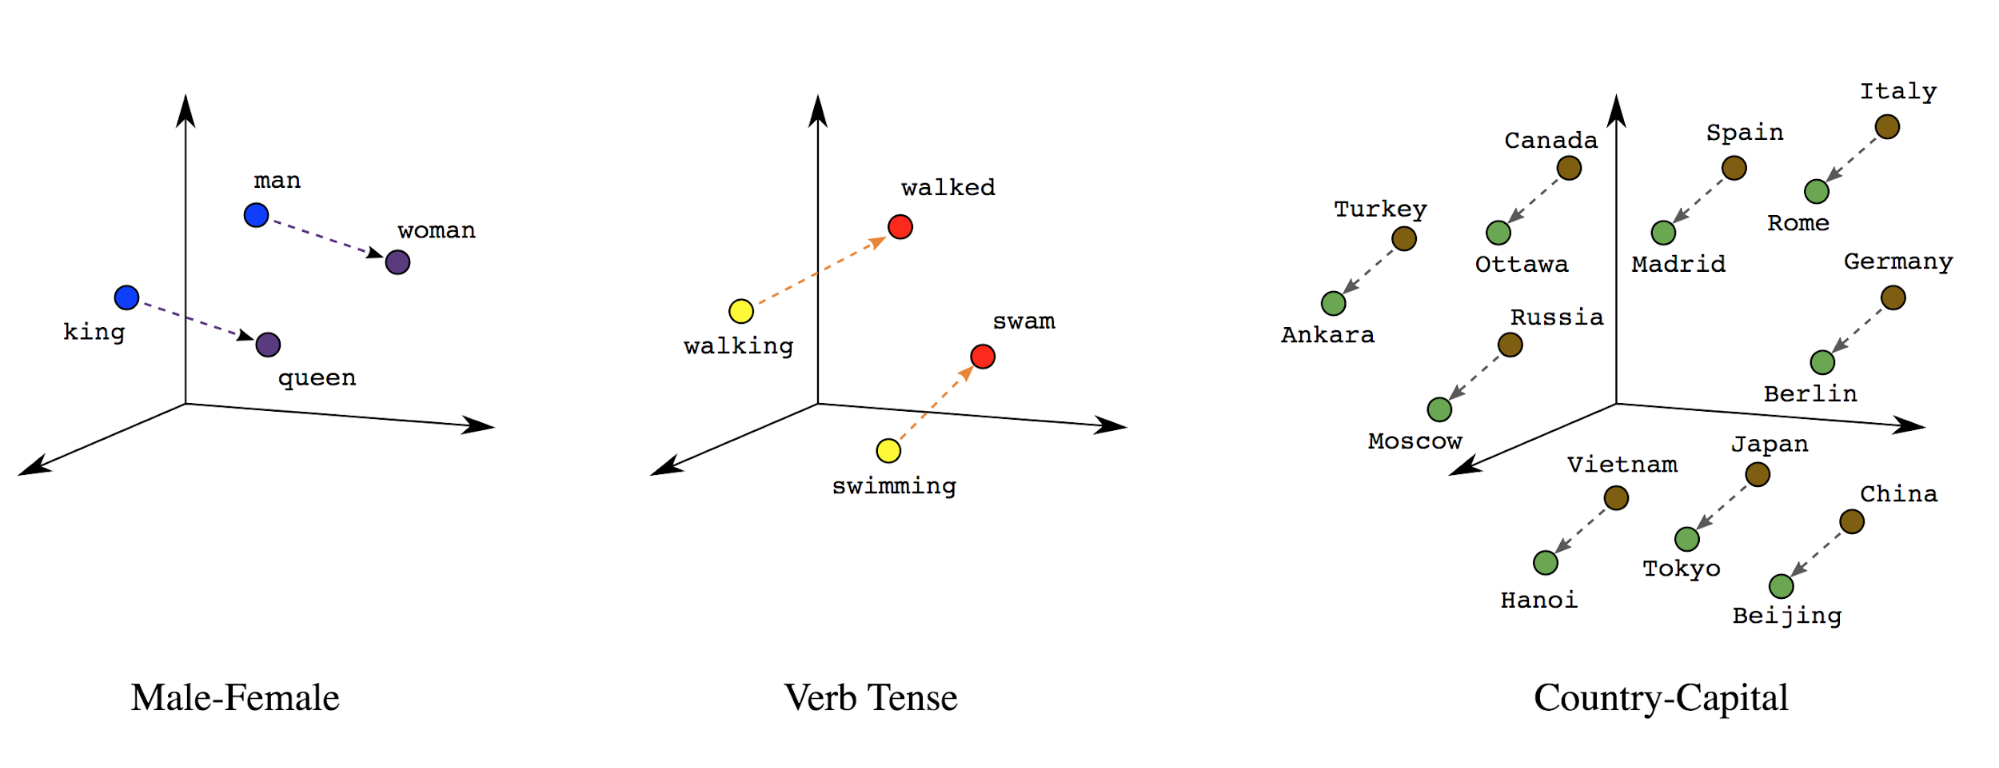
\includegraphics[width=0.8\textwidth]{images/wordvec.png}
	\caption{Exemple de relations entre vecteurs sémantiques}
	\label{wordvec}
\end{figure}

Ces vecteurs sont générés par un processus relativement simple quand on connait les bases de l'\gls{ml}. Je vais brièvement expliquer ici deux méthodes, présentées en plus de détail dans le papier word2vec \cite{word2vec}. La figure \ref{word2vec} décrit les structures des modèles présentés, qui sont en fait symétriques l'un de l'autre.

\begin{figure}[ht]
	\centering
	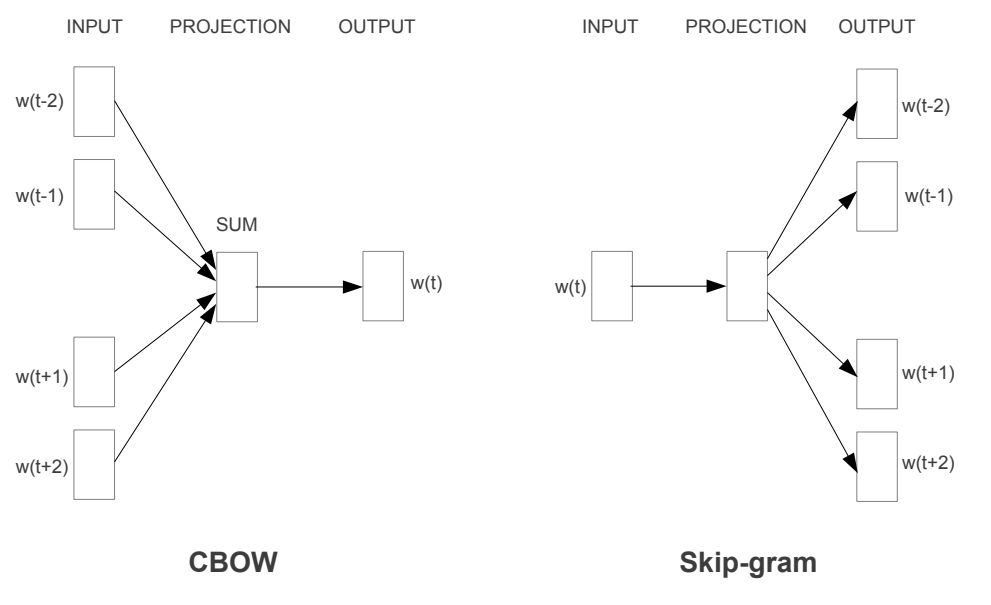
\includegraphics[width=0.7\textwidth]{images/word2vec.png}
	\caption{Architectures de vectorisation de word2vec}
	\label{word2vec}
\end{figure}

Chacune de ces méthodes utilise les vecteurs sémantiques comme entrée et sortie du réseau, et au début de l'entrainement chaque mot est lié a un vecteur aléatoire. En utilisant un corpus de texte, un mot ainsi que les mots qui l'entourent sont utilisés pour améliorer les valeurs du vecteur du mot central. Pour le CBOW (Continuous Bag Of Words, ou sac de mots continu), le <<contexte>> autour du mot est donné, et on entraine le réseau a deviner le mot actuel. À l'inverse, pour le modèle skip gram, on donne le mot initial et on fait deviner les mots qui l'entourent.

Cette méthode présente des résultats très concluants, et de nombreuses méthodes plus récentes s'en inspirent pour résoudre des problèmes similaires. Pour les utiliser en pratique, il n'est pas réellement nécessaire de refaire toute cette procédure d'entrainement. Il suffit de récupérer une sorte de dictionnaire, qui affecte a chaque mot son vecteur sémantique. Il existe de ces dictionnaires pour beaucoup de langages, et notamment en français. Il est important de noter que certains contextes nécessiteraient de ré-entrainer un modèle, mais c'est très rare.

\todo{Tester fonctionnement \href{http://nlp.polytechnique.fr/word2vec}{Polytechnique NLP}}

\section{Forêt d'isolation}

La forêt d'isolation, décrite en 2009 \cite{isolationforest}, est une méthode d'\gls{ml} classique utilisée pour la détection de valeurs aberrantes. Elle fonctionne en déterminant un coefficient d'isolation pour chaque valeur d'un jeu de données, déterminée par la facilité a la séparer du reste des données.

L'algorithme est exécuté de cette façon:

\begin{enumerate}
	\item On choisit aléatoirement une variable (exemple, $x$ ou $y$ en 2 dimensions)
	\item On choisit une valeur de seuil aléatoire, entre le maximum et le minimum de cette variable dans les points non isolés
	\item On sépare les points inférieurs et supérieurs a ce seuil
	\item Si un point de donnée se retrouve isolé du reste, on ne le compte plus pour l'algorithme, et on mémorise le nombre de <<splits>> qu'il a fallu faire pour l'isoler
	\item Si tous les points n'ont pas été isolés, on retourne à l'étape 1.
\end{enumerate}

A la fin de cette boucle, un score d'isolation compris entre 0 (valeur normale) et 1 (anomalie) est calculé en fonction du nombre de splits. L'algorithme utilisant de l'aléatoire, il est possible de l'exécuter plusieurs fois pour obtenir une valeur moyenne d'isolation pour chaque point. Un exemple de séparation pour un point normal et aberrant est montré en figure \ref{isoforest}.

\begin{figure}[ht]
	\centering
	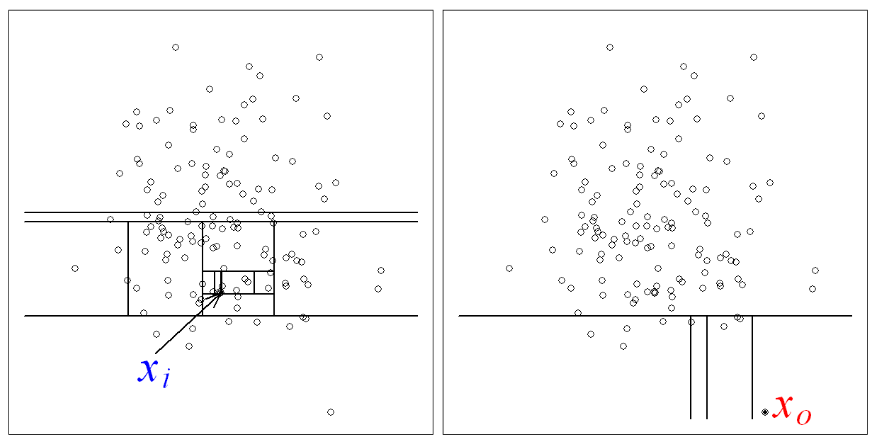
\includegraphics[width=0.7\textwidth]{images/isoforest.png}
	\caption{Fonctionnement des forêts d'isolation}
	\label{isoforest}
\end{figure}

\newpage
\chapter{L'existant: le projet analyse-logs}

\section{Contexte du projet}

Si le premier chapitre peut mettre quoi que ce soit en avant, c'est bien le besoin très fort en informatique de la \gls{DGFiP}, rempli par le \gls{SI} et ses très nombreuses applications. Mais un parc applicatif si étendu pose un problème majeur~: celui de la maintenance. En effet, la maintenance logicielle est un processus très coûteux, surtout en termes d'heures de travail de personnes qualifiées. Ce sont les développeurs des applications à maintenir qui doivent effectuer cette maintenance, car c'est eux qui connaissent le fonctionnement interne de l'application.

Une solution serait de former des équipes de maintenance au différents logiciels. Malheureusement, cela demanderait encore plus de moyens, à la fois prenant encore du temps aux développeurs, mais aussi nécessitant d'embaucher des personnes qui travailleraient a temps plein sur la maintenance, ce qui n'est pas envisageable. Il n'est même pas donné que cela libère vraiment du temps aux développeurs, étant donné l'évolution constante des logiciels et les formations supplémentaires qu'il faudrait donner pour tenir une équipe de maintenance à jour.

\bigskip
Il y a 4 ans, mon tuteur Olivier Blanc s'est penché sur la question. Le vrai problème était bien de faire gagner du temps aux développeurs en facilitant et accélérant la maintenance d'une application. Dans le cas d'une erreur dans l'application qui stopperait partiellement ou complètement son fonctionnement, sa correction est obligatoire pour les équipes. Le problème de retrouver la source de cette erreur et de la corriger est alors aussi important, et c'est ici que rentrent en jeu les \glspl{log} applicatifs (voir partie suivante). Olivier mit en avant le papier de recherche DeepLog \cite{deeplog}, dont le but était d'utiliser les logs pour détecter et prédire les erreurs, ainsi que remonter vers leur cause initiale. Le projet \texttt{analyse-logs} est alors né, commençant comme sujet de PFE de Rémi Grison, apprenti a la DGFiP en 2019. Léa Lebert à ensuite succédé à Rémi, puis un an après le départ de Léa j'ai repris le projet.

\section{Le modèle original: DeepLog}

Le travail de Rémi qui a démarré ce projet a principalement été l'implémentation de l'algorithme DeepLog à partir du papier de Du et al. \cite{deeplog}. Je vais ici détailler le fonctionnement de DeepLog ainsi que l'implémentation qui a été faite par Rémi.

\begin{figure}[ht]
	\centering
	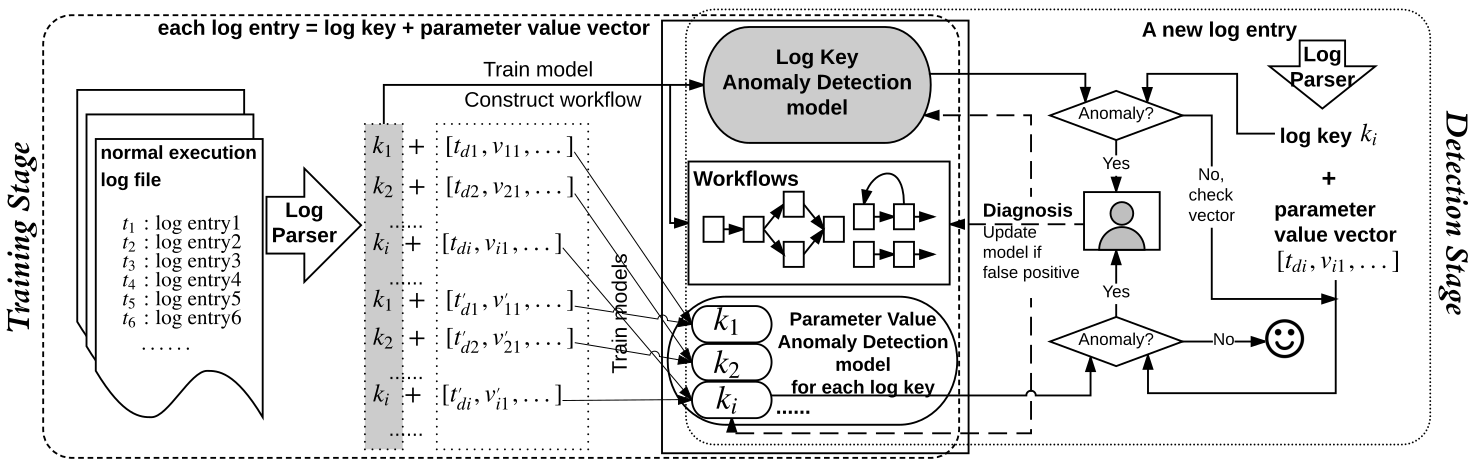
\includegraphics[width=\textwidth]{images/deeplog.png}
	\caption{Structure de DeepLog}
	\label{deeplog}
\end{figure}

La structure complète du modèle est détaillée dans la figure \ref{deeplog}, tirée directement du papier. Une étape qui n'est pas détaillée ici est celle de la récupération et du regroupement des \glspl{log}, qui n'est pas aussi triviale qu'elle pourrait en avoir l'air. Cependant, ce point ne sera pas plus approfondi dans ce rapport étant donné que nous ne l'avons pas vraiment traité.

\subsection{Parsing}

La première étape est celle du <<parsing>> (que l'on pourrait approximativement traduire par analyse syntaxique en français). Elle est appliquée a un fichier de \glspl{log} pour le traduire en une liste d'ids et de vecteurs de paramètres. Par exemple, avec les \glspl{log} suivant:

\begin{lstlisting}
Session ouverte id 123
Session ouverte id 456
Session fermée id 123
Session fermée id 456
\end{lstlisting}

On s'attend a obtenir un tel résultat parsé:

\begin{lstlisting}
1, [123]
1, [456]
2, [123]
2, [456]
\end{lstlisting}

La méthode utilisée par DeepLog pour produire ces résultats est Spell \cite{spell}, développée l'année précédente par une partie des chercheurs qui ont travaillé sur DeepLog. Seulement, entre la publication du papier et l'implémentation par Rémi, 2 années sont passées, et l'état de l'art avait changé en faveur de l'algorithme Drain \cite{drain}. Cet algorithme avait été publié la même année que DeepLog, et est encore aujourd'hui une solution de choix pour le parsing de \glspl{log}. Rémi a donc produit sa propre implémentation de l'algorithme Drain pour le projet. Il existe aujourd'hui une très bonne implémentation open source de drain en Python, qui est donc plus robuste et performante que l'implémentation de Rémi, et nous allons donc la réutiliser plus tard.

\subsection{Analyse des suites}

L'étape d'analyse de DeepLog est séparée en deux parties. Les chercheurs de DeepLog avaient pour but de créer un modèle plus puissant que ce qui a pu exister auparavant. Un des problèmes de ces anciens modèles est l'absence de prise en compte de la temporalité, les \glspl{log} étant seulement analysés un par un sans prendre en compte leur ordre d'apparition. L'analyse de l'enchaînement des \glspl{log} est donc très importante pour mieux comprendre certaines erreurs moins évidentes à premier abord.

\begin{figure}[ht]
	\centering
	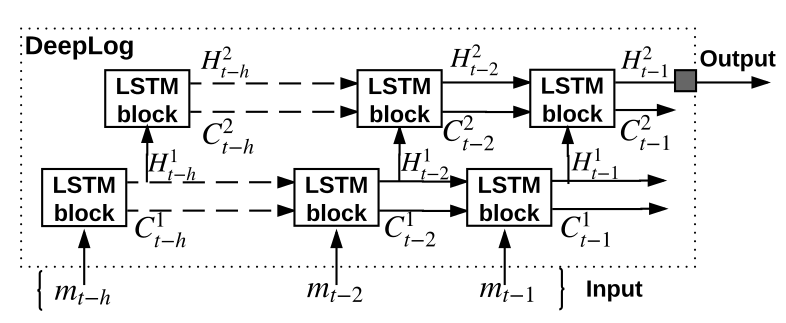
\includegraphics[width=0.6\textwidth]{images/stacked_lstm.png}
	\caption{Structure d'un réseau LSTM empilé}
	\label{lstm}
\end{figure}

L'analyse temporelle est faite par DeepLog à l'aide de réseaux \gls{LSTM} empilés (voir figure \ref{lstm}). Un \gls{LSTM} est un type de réseau de neurones en \gls{deep}, qui possède des connections de rétroaction qui lui permettent de capturer des comportements sur une durée relativement longue.

Les ids des \glspl{log} sont utilisés, et on entraine le modèle à prédire les $g$ \glspl{log} les plus probables qui apparaitraient après une suite de $h$ \glspl{log}, à l'aide d'une fenêtre glissante. Par exemple, pour cet enchainement d'ids: \texttt{1, 2, 1, 3, 4, 1, 2}, avec une taille de fenêtre $h=5$, on va envoyer \texttt{1, 2, 1, 3, 4} au réseau, et on s'attend a voir \texttt{1} au sein des $g$ \glspl{log} prédits. Ensuite on enverrait \texttt{2, 1, 3, 4, 1} en attendant \texttt{2}, etc.

\bigskip
Cet entraînement pourra ensuite être utilisé durant l'analyse d'un fichier de \glspl{log}, ou même durant son exécution. On prévoit les $g$ ids les plus probables, puis on compare avec le \gls{log} qui est vraiment à la suite. Si son id n'est pas dans les prédictions de l'algorithme, on considère ce log comme anormal.

\subsection{Analyse des paramètres}

Le choix des créateurs de DeepLog a été de considérer chaque partie variable des \glspl{log} (soit chaque paramètre) comme sa propre série temporelle à travers les \glspl{log} de même id. En faisant cela, il est possible de réutiliser la même architecture de \gls{LSTM} empilés détaillés a la figure \ref{lstm}. Cette fois, on attend une unique prédiction de valeur, et les lignes sont considérées comme anormales si la valeur observée est trop différente de la valeur réelle.

\section{Evolutions du projet par Léa}

Suite à l'implémentation de DeepLog par Rémi, le projet était certes fonctionnel mais très peu utilisable par un utilisateur lambda. En effet, l'utilisation se faisait à travers une ligne de commande comportant de nombreux paramètres, celle-ci étant la seule interface pour les utilisateurs.

Le travail de Léa a donc été d'améliorer ce projet pour le rendre plus simple d'utilisation, mais aussi d'agrandir l'éventail de possibilités d'analyse proposé. Il a été choisi de créer une nouvelle façon de faire l'interface avec le modèle via la bibliothèque Blockly créée par Google, détaillée à la suite. Je ferai aussi une explication des autres algorithmes mis en place, sur quoi j'avais aidé Léa au moment de son PFE.

\subsection{Blockly}

\begin{figure}[ht]
	\centering
	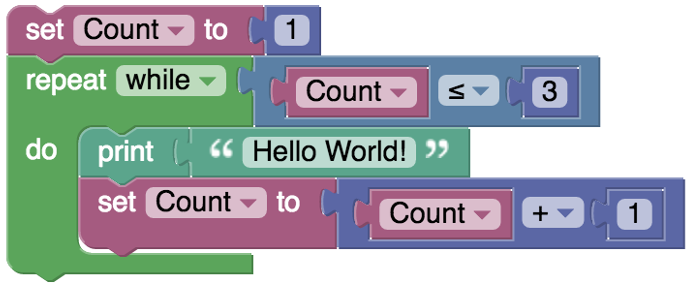
\includegraphics[width=0.4\textwidth]{images/blockly.png}
	\caption{Exemple de programme avec Blockly}
	\label{blockly}
\end{figure}

Blockly est une librairie publiée par Google, permettant de créer des éditeurs de code visuels. L'utilisateur relie des blocs qui représentent des instructions, des variables, des boucles (voir figure \ref{blockly}) et cette représentation est traduite en code, de façon entièrement configurable par un développeur. Si vous avez déjà eu affaire au moteur de jeu en ligne Scratch, son éditeur visuel est basé sur Blockly.

\bigskip
Olivier et Léa ont fait le choix d'utiliser cette librairie pour représenter les différentes structures de modèles, ou <<pipelines>>. En effet, si on considère chaque bloc du modèle, il est possible de les remplacer par d'autres blocs équivalents, par exemple un autre analyseur de modèle. Blockly permet très bien cette représentation, avec des couleurs et des formes qui correspondent aux types des éléments. Chaque étape du modèle pourrait alors avoir son type de bloc, et l'interface serait visuellement très intuitive.

L'interface Blockly a donc été développée par dessus le travail de Rémi, mais aussi avec les autres algorithmes détaillés dans la partie suivante. Elle n'aurait eu que peu d'intérêt si l'idée d'algorithmes/modèles alternatifs n'avait pas été émise, mais cette idée permet de créer facilement et intuitivement des modèles adaptés aux besoins de différentes applications de la DGFiP.

\subsection{Algorithmes alternatifs}

Il existe de nombreux algorithmes qui, a partir de suites d'ids ou de paramètres, seraient capables de prévoir la validité d'une occurrence suivante. En effet, une partie de la force de DeepLog repose dans son architecture très modulaire, et il serait donc envisageable de remplacer une étape par une autre similaire.

Le premier algorithme qui a été choisi est les <<forêts d'isolation>> \cite{isolationforest}, qui se base sur une valeur d'isolation d'un point de données: plus il est facile de le séparer du reste des données, plus il a de chances d'être une anomalie (voir section \ref{isoforest}). Un module d'analyse de paramètre a été développé avec une implémentation des forêts d'isolation, capable de remplacer celui de DeepLog dans l'implémentation de Rémi.

\bigskip
C'est ici que j'ai eu mon premier contact avec le projet durant ma première année d'alternance. Il m'a fallu assister Léa sur la fin de son PFE, pour effectuer des tâches qu'elle n'avait pas le temps de faire. J'ai aussi pu apporter une aide technique sur la partie \gls{ml} du projet, étant suite a avoir suivi un cours a ce sujet.

En m'inspirant de ce qui a été fait sur les forêts d'isolation, j'ai fait le choix de créer un module d'analyse de suites et de paramètres générique basé sur la librairie d'\gls{ml} scikit learn. C'est une bibliothèque libre présentant de nombreux algorithmes communs d'\gls{ml}, tels que les forêts d'isolation. Utiliser une librairie telle que scikit me permet tout d'abord une meilleure robustesse et performance des algorithmes, mais aussi une certaine généricité. En effet, les algorithmes du même type ont tous la même structure de fonctions, et cela permet de très facilement les interchanger.

Les modules qui ont été développés permettent donc de remplacer l'analyse de paramètres de DeepLog par n'importe quel algorithme de la bibliothèque scikit, s'intégrant parfaitement dans la structure par blocs proposée par Blockly. Trois algorithmes de détections d'anomalies ont été retenus: les forêts d'isolation (version scikit), les SVM (Support Vector Model, ou \link{https://fr.wikipedia.org/wiki/Machine_à_vecteurs_de_support}{Séparateur à Vaste Marge}) à une classe, et les LOF (\link{https://en.wikipedia.org/wiki/Local_outlier_factor}{Local Outlier Factor}). Ce sont trois méthodes de l'état de l'art en apprentissage non profond pour la détection d'anomalie, qui pourraient s'avérer utiles pour l'analyse de paramètres en particulier.

\newpage
\chapter{Le processus scientifique au cœur du projet}

Nous arrivons maintenant au cœur de ce mémoire, qui démarre au début de mon PFE, et plus précisément l'arrivée de Robin à la \gls{DGFiP}. Robin était étudiant en Master ALMA à l'université de Nantes, et a travaillé avec moi sur le projet d'analyse de \glspl{log} en tant que sujet de stage de fin de master. Il s'est chargé de beaucoup de travail de documentation sur le sujet ainsi que des sujets plus axés recherche.

Je vais détailler au sein de ce chapitre cette grande partie du projet et les différents points important que nous avons rencontrés.

\section{État de l'art de l'analyse de logs}

À l'arrivée de Robin au bureau, j'étais encore en période école. Il a donc commencé le travail sur le projet avant moi, et ce en commençant la rédaction d'un état de l'art des algorithmes d'analyse de \glspl{log} existants. Ce travail est un travail de longue haleine, la compréhension des papiers n'étant pas du tout triviale. Malgré les meilleurs efforts des chercheurs les ayant rédigés, un long travail de documentation et d'apprentissage est nécessaire pour comprendre certains des concepts abordés et utilisés.

Un papier qui a beaucoup aidé cette recherche documentaire est le rapport d'expérience \cite{experiencereport} publié par Huawei et l'université de Hong Kong en 2021. Ce document étant très récent, étant publié environ 6 mois avant le début du projet, il nous a semblé être une source fiable d'informations et de données au sujet de la détection d'anomalies dans les logs. Il compare notamment DeepLog à cinq autres méthodes, pour un total de trois méthodes (semi-)supervisées et trois non-supervisées.

Nous avons eu beaucoup d'échanges avec Robin durant ses recherches documentaires, au sujet des algorithmes trouvés, de détails incompris ou de points intéressant. Nous avons pu comme cela mieux comprendre les différents papiers trouvés, et faire des choix et des hypothèses au sujet de l'implémentation et des résultats.

\bigskip
Cette recherche nous a mené à choisir les algorithmes que nous souhaitions implémenter pour la suite, que je vais détailler dans la suite de cette section. Nous avons choisi ces algorithmes en fonction de notre compréhension des mécanismes en jeu, de leur facilité d'implémentation perçue, ainsi que de leur utilité vis à vis de notre problème.

\subsection{LogRobust}

\begin{figure}[ht]
	\centering
	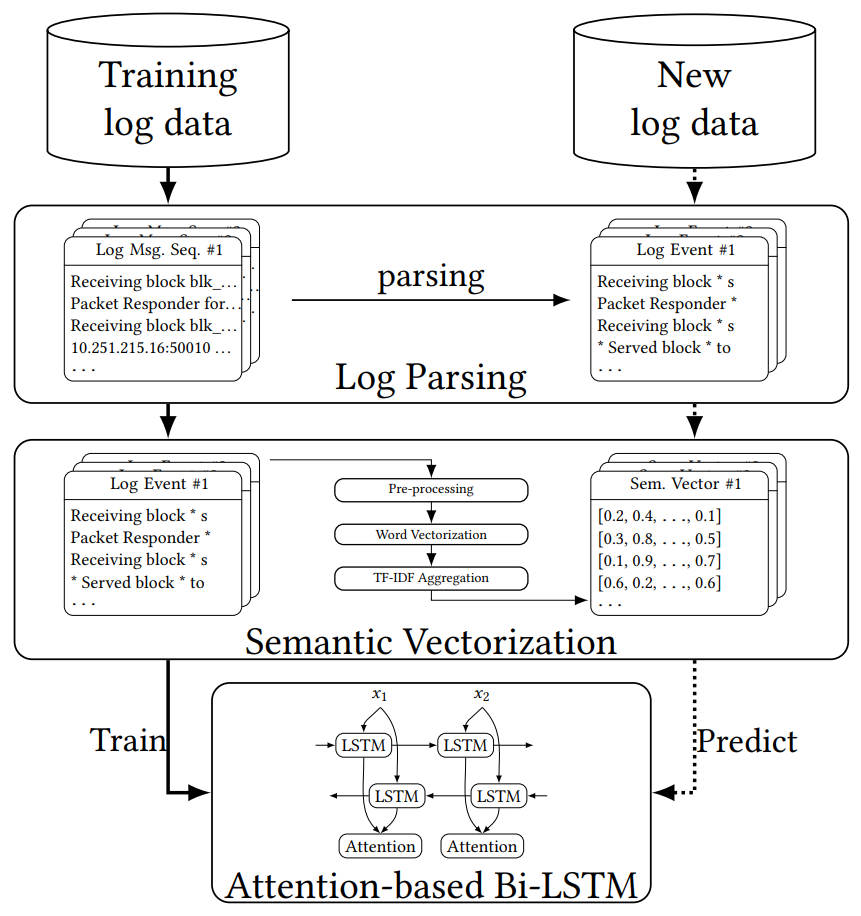
\includegraphics[width=0.4\textwidth]{images/logrobust.png}
	\caption{Structure de LogRobust}
	\label{logrobust}
\end{figure}

LogRobust \cite{logrobust} est un modèle d'analyse de \glspl{log} qui montre des similarités avec DeepLog, publié en 2019. Comme son nom l'indique, l'objectif était de pallier aux problèmes des anciennes méthodes de l'état de l'art en proposant une solution robuste. L'architecture du modèle est détaillée sur la figure \ref{logrobust}.

\bigskip
La plus grosse différence de ce modèle comparé à DeepLog est l'étape de vectorisation sémantique présente à la suite du parsing. Si DeepLog utilise les id de \glspl{log} et les valeurs des différents paramètres pour reconnaître les anomalies, LogRobust utilise la sémantique des \glspl{log} et leur enchaînement (voir section \ref{vectorisationsemantique} pour plus de détails). Cette analyse sémantique permet effectivement de lisser les valeurs utilisées, d'où la promesse de robustesse de l'algorithme. Des lignes ayant la même signification, par exemple un log dans lequel des synonymes ont été remplacés dans une mise à jour, resteront proche, et ne nécessiteront pas un ré-entrainement du modèle.

\begin{figure}[ht]
	\centering
	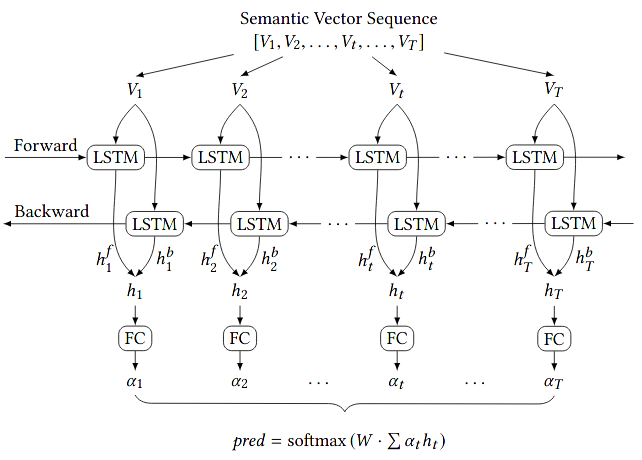
\includegraphics[width=0.6\textwidth]{images/bilstm.png}
	\caption{Structure d'un LSTM bidirectionnel}
	\label{bilstm}
\end{figure}

\bigskip
Une autre différence notable comparé à DeepLog est l'utilisation d'un bi-\gls{LSTM} avec un mécanisme d'attention (voir figure \ref{bilstm}). Le fonctionnement d'un bi-\gls{LSTM} est similaire au \gls{LSTM} utilisé par DeepLog, mais on en utilise un dans le sens chronologique (comme DeepLog) et un dans le sens inverse, avec des entrées allant du futur vers le passé. Cela permet de rajouter un contexte temporel aux \glspl{log}, ce qui améliore en général les performances. Un problème posé par cette approche est la nécessité de connaitre un certain nombre d'entrées dans le futur, et dans le cas d'une analyse en direct un délai supplémentaire est alors nécessaire.

Le mécanisme d'attention simule le concept d'attention humain. Par exemple, quand on lit une phrase, on est capable de savoir quel mots lus précédemment sont important relativement au mot que l'on lit maintenant. C'est ce que fait LogRobust avec les \glspl{log}, en apprenant au fur et à mesure quel \glspl{log} de l'historique sont importants vis à vis du log analysé.

\bigskip
La robustesse du modèle est testée en modifiant les fichiers de logs de différentes façons, de manière aléatoire:

\begin{itemize}
	\item En modifiant les clés des \glspl{log}:
	\begin{itemize}
		\item Ajout de mots et/ou de paramètres
		\item Suppression de mots
	\end{itemize}
	\item En modifiant l'enchaînement des \glspl{log}:
	\begin{itemize}
		\item Suppression de \glspl{log}
		\item Mélange de \glspl{log}
		\item Duplication de \glspl{log}
	\end{itemize}
\end{itemize}

Ces fichiers de \glspl{log} modifiés sont ensuite utilisés par les chercheurs pour évaluer la robustesse du modèle LogRobust. Comparé a des méthodes d'\gls{ml} classiques (non profond), les performances sont très concluantes. En effet, la méthode performe bien face à des niveaux d'injection jusqu'à 20\%, et l'attention est mise en valeur car elle permet de garder les résultats corrects à des niveaux d'injection élevés.

\bigskip
Cette méthode serait donc une très bonne méthode a implémenter pour être durable dans le temps. Il n'est pas nécessaire de la ré-entrainer fréquemment (ce qui pouvait être un problème avec DeepLog. Il est important de noter que cette méthode ne prend pas en compte les valeurs des paramètres des \glspl{log}, ce qui pourrait être un problème dans certains cas d'application. Mais la robustesse de la méthode liée a son mécanisme d'attention, ainsi que son architecture relativement simple, sont de bons arguments pour son utilisation.

\subsection{AutoEncoder}

Cette méthode publiée en 2020 \cite{autoencoder} est appelée <<AutoEncoder>> dans le reste du document, mais elle utilise en réalité 2 réseaux de type autoencoder ainsi que des forêts d'isolation.

\begin{figure}[ht]
	\centering
	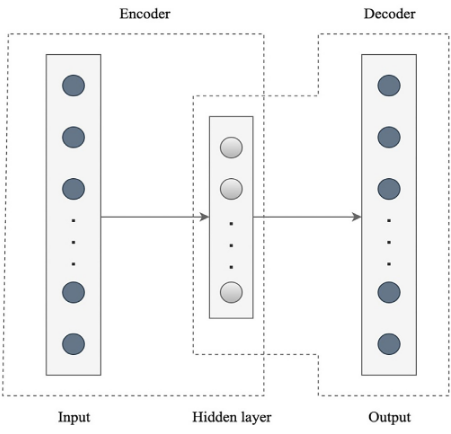
\includegraphics[width=0.6\textwidth]{images/autoencoder.png}
	\caption{Structure d'un réseau autoencoder}
	\label{autoencoder}
\end{figure}

\bigskip
Le plus important pour comprendre ce modèle est le fonctionnement d'un AutoEncoder. C'est encore une fois un réseau de neurone, avec une structure simple en <<double entonnoir>> (voir figure \ref{autoencoder}). L'objectif de cette structure est d'apprendre un encodage (et décodage) de données pour réduire la taille de cette donnée, avec une perte d'information minimale. La valeur encodée est donc ce que l'on va retrouver dans la couche cachée au centre du réseau, et notre apprentissage nous permet d'encoder et de décoder des données par la suite.

\begin{figure}[ht]
	\centering
	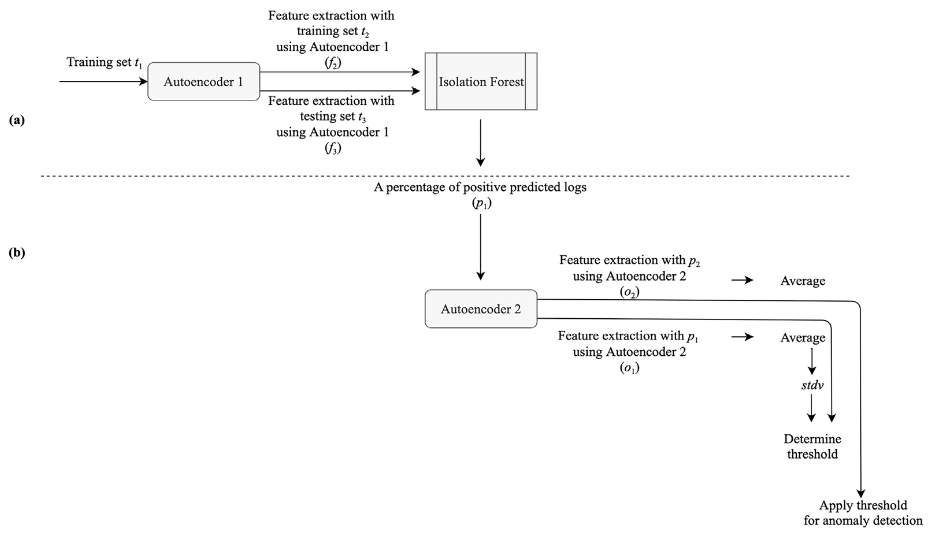
\includegraphics[width=\textwidth]{images/modeleautoencoder.png}
	\caption{Structure du modèle <<AutoEncoder>>}
	\label{modeleautoencoder}
\end{figure}

\bigskip
La structure complète du modèle est détaillée dans la figure \ref{modeleautoencoder}. Le premier autoencoder est entrainé à encoder les \glspl{log}, soit en extraire les variables significatives. Ensuite, la forêt d'isolation fait une première passe de détection d'anomalies selon ces \glspl{log} encodés, ce qui à la fois accélère le processus et améliore la détection. Enfin, une seconde passe de détection d'anomalies est faite avec un second autoencoder, qui va récupérer à la fois les valeurs négatives détectées par la forêt d'isolation et les valeurs positives. Cette passe permet de déterminer et utiliser un seuil d'acceptation des \glspl{log}.

C'est une structure très complexe, et je ne saurais décrire en détail les raisons de sa structure si particulière. Mais c'est une méthode qui n'est pas trop compliquée a mettre en place malgré tout, se basant sur des concepts bien connus et implémentés dans des librairies, qu'il suffit de composer. Les résultats détaillés dans le papier sont assez concluants, et les comparaisons du rapport d'expérience \cite{experiencereport} montrent qu'il est notamment très robuste pour des jeux de données avec beaucoup d'anomalies, ce qui n'est pas le cas des autres modèles.

\section{Analyse des jeux de données disponibles}

Nous avons réussi à obtenir un large jeu de données de \glspl{log} de l'application \gls{MEDOC} dont j'ai parlé succinctement dans la section \ref{dgfip}. Elle produit une grosse quantité de \glspl{log} liés notamment aux parcours utilisateurs durant leur sessions sur l'application. Voici un exemple de \gls{log} tiré de ce jeu de données:

\begin{lstlisting}
2021-05-14 07:35:17,106 - http-bio-8140-exec-32 - INFO -
| fr.gouv.finances.medoc.persistance.cpl.dao.VerrouDao.
| leverVerrousUtilisateur(VerrouDao.java:167) - 0 Supprimés pour
| la session SERV0070100-AG323056-0DB4EE01F8D31E5C4D2EE3BDA6131B62
\end{lstlisting}

On retrouve ici les différents éléments abordés dans la section \ref{logs}, tels que la date, l'heure et le niveau du \gls{log}. Seulement, on retrouve aussi des informations supplémentaires telles que le fil d'exécution, la classe et la méthode d'origine. Ce sont des informations supplémentaires qui peuvent être très utiles à un développeur pour tracer l'origine d'une erreur.

\bigskip
De nombreux \glspl{log} comportent aussi un identifiant de session, par exemple le long identifiant lisible a la fin de la ligne d'exemple ci-dessus. La gestion des sessions est un point très important dans l'analyse de \glspl{log}, en particulier quand on prend en compte l'enchainement des \glspl{log} comme le font DeepLog et LogRobust. En effet, si les sessions se retrouvent entrelacées dans les \glspl{log}, les enchainements peuvent devenir imprévisibles, et une anomalie peut être détectée là où il n'y en a pas.

Il existe plusieurs solutions à ce problème d'entrelacement:
\begin{itemize}
	\item Désentrelacer les \glspl{log}: Si tous les \glspl{log} appartenant à des sessions différentes contiennent un identifiant de sessions et que son extraction est possible, il est possible de les désentrelacer. Il serait alors envisageable de traiter les sessions une par une, ou bien de les regrouper au sein même du flux des \glspl{log}.

Cette solution pose certains problèmes qui nécessiterait des changements de structure des modèles, notamment pour la gestion de successions des \glspl{log} avec des heures qui ne se suivent pas.

	\item Augmenter la taille de l'historique: L'analyse se fait avec un historique de \glspl{log} d'une taille fixe, à partir du quel on prévoit le log suivant. Si cet historique est grand, précisément plus grand que la taille totale des sessions entrelacées, l'algorithme serait capable de ne prendre en compte que les \glspl{log} intéressants de cet historique. Cela est d'autant plus vrai pour un système implémentant un mécanisme d'attention.
\end{itemize}

La solution la plus évidente à mettre en place serait donc la seconde. Un point crucial est donc de connaitre ces tailles de session dans nos jeux de données de \gls{MEDOC}, et d'autres données tirées de ces \glspl{log} pourraient aussi nous être utiles.

\bigskip
Une analyse des données a donc été mise en place via un notebook Python Jupyter, comme nous avions utilisé cet outil en cours pour ce même genre de tâches. Un notebook permet de séparer du code Python en différents blocs exécutables séquentiellement et séparément, ce qui est utile pour du traitement de données et des visualisations.

\begin{figure}[ht]
	\centering
	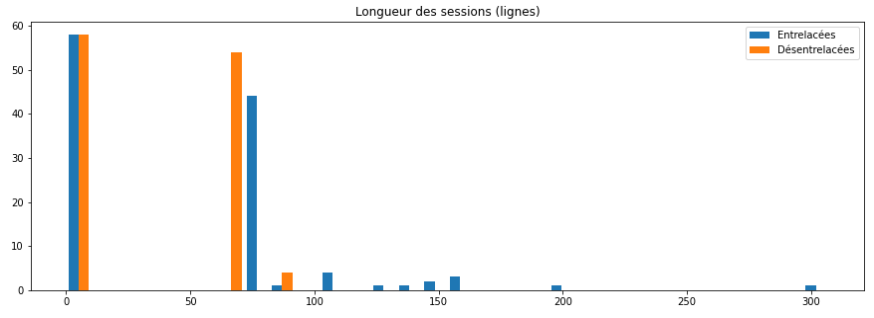
\includegraphics[width=\textwidth]{images/longsess.png}
	\caption{Longueur des sessions dans les logs MEDOC}
	\label{longsess}
\end{figure}

La première donnée sortie de cette analyse est la longueur des sessions, entrelacées ou non pour permettre une comparaison (figure \ref{longsess}). Cette première analyse amène déjà beaucoup d'informations sur le comportement des sessions. D'abord, on observe de nombreuses sessions contenant un unique \gls{log}, ce qui est un peu suspect et qu'il faudra étudier par la suite. Ensuite, l'entrelacement des sessions est assez minime mais cause quand même une explosion de la longueur maximale de session: une session passe ici de moins de 100 lignes à elle seule, a 300 lignes quand entrelacée avec le reste des \gls{log}. Enfin, on observe aussi l'existence d'une session qui comporte plus de 1000 lignes quand désentrelacée.

\begin{figure}[ht]
	\centering
	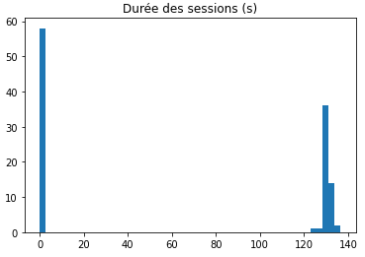
\includegraphics[width=0.4\textwidth]{images/dureesess.png}
	\caption{Durée des sessions}
	\label{dureesess}
\end{figure}

Une autre analyse qui a été effectuée est celle de la durée dans le temps des sessions (voir figure \ref{dureesess}). On retrouve ici les sessions qui ne contiennent qu'un unique \gls{log}, et ont une durée nulle. Sinon, on peut observer que les sessions ont une durée très proche, autour de 2 minutes 10 secondes.

\bigskip
Une analyse plus détaillée des sessions de 1 ligne nous indique qu'elles sont toute, sans exceptions, des sessions <<Catalina>>. En effet, les autres sessions comportent toutes au minimum un message d'ouverture et de fermeture de session, et des traitements sont toujours effectués entre ces deux évènements. Mais que sont ces sessions Catalina? Catalina est un composant de Tomcat, le moteur de serveur utilisé à la DGFiP. Catalina est en fait l'implémentation du moteur de Tomcat, ou plus précisément des <<servlets>> Tomcat (voir article wikipédia \link{https://fr.wikipedia.org/wiki/Servlet}{Servlet} pour plus d'informations). Ces \glspl{log} représentent des fermetures de sessions Catalina, qui ne sont a priori pas les mêmes que les sessions utilisateurs qui nous intéressent.

Tout ce qu'il nous faut savoir, c'est que ces sessions ne sont pas très intéressantes à mettre à part du reste des \glspl{log}. Heureusement, tous ces \glspl{log} ont la même structure:

\begin{lstlisting}
2021-05-14 08:06:16,078 -
| ContainerBackgroundProcessor[StandardEngine[Catalina]]
| - INFO - fr.gouv.finances.commun.jee9.mapi.presentation.session.
| BasicSessionListener.sessionDestroyed(BasicSessionListener.java:92)
| - Destruction de session '<id>'
\end{lstlisting}

Ce sont les seuls \glspl{log} originaires du fil d'exécution \texttt{ContainerBackgroundProcessor\allowbreak [Stan\-dard\allowbreak Engine[Catalina]]}, il est alors possible de s'en servir comme filtre et de retirer ces \glspl{log} de l'analyse des sessions, présenté en figure \ref{longsesscata}.

\begin{figure}[ht]
	\centering
	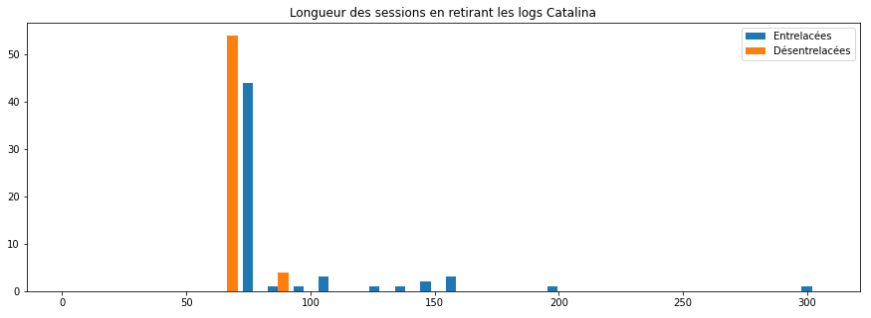
\includegraphics[width=\textwidth]{images/longsesscata.png}
	\caption{Longueur des sessions en retirant les logs Catalina}
	\label{longsesscata}
\end{figure}

Une dernière analyse effectuée est celle de la composition des \glspl{log}. Le fichier de \glspl{log} utilisé n'est qu'un extrait de tout le jeu de données auquel nous avons accès, par souci de performance. Mais cette analyse nous permet quand même de détailler la structure des \glspl{log} avec lesquels nous devons travailler. La figure \ref{proportionsess} détaille les pourcentages de \glspl{log} appartenant a une session, ainsi qu'une session Catalina.

\begin{figure}[ht]
	\centering
	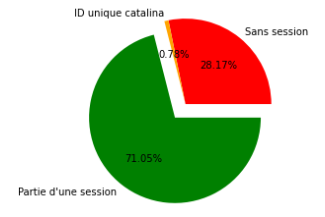
\includegraphics[width=0.4\textwidth]{images/proportionsess.png}
	\caption{Proportions de logs appartenant à des sessions}
	\label{proportionsess}
\end{figure}

\newpage
\chapter{Développement du nouveau projet}

Durant la partie scientifique du projet, et ayant déjà travaillé sur le projet de Rémi et Léa, différents points d'évolutions sont devenus apparents. Le projet est très large, et il ressemble à un projet auquel on aurait rajouté des modules au fur et à mesure sans vraiment de planification au départ, ni de temps passé a repenser cette structure. Le problème qui se pose ici est celui de la dette technique, qui s'accumule sur les projets a grande échelle si elle n'est pas prise en compte.

J'ai alors fait le choix de faire une réécriture du projet, et surtout de repenser entièrement son architecture. L'objectif était de la rendre flexible aux changements et surtout ajouts, pour permettre au projet de grandir et évoluer avec les différents projets qui l'utiliseraient dans le futur. Principalement, on doit être capable d'aisément ajouter des algorithmes différents proposant différentes analyses et caractéristiques, pour le futur du projet mais aussi et surtout pour pouvoir nous les implémenter et tester plus facilement.

\begin{figure}[ht]
	\centering
	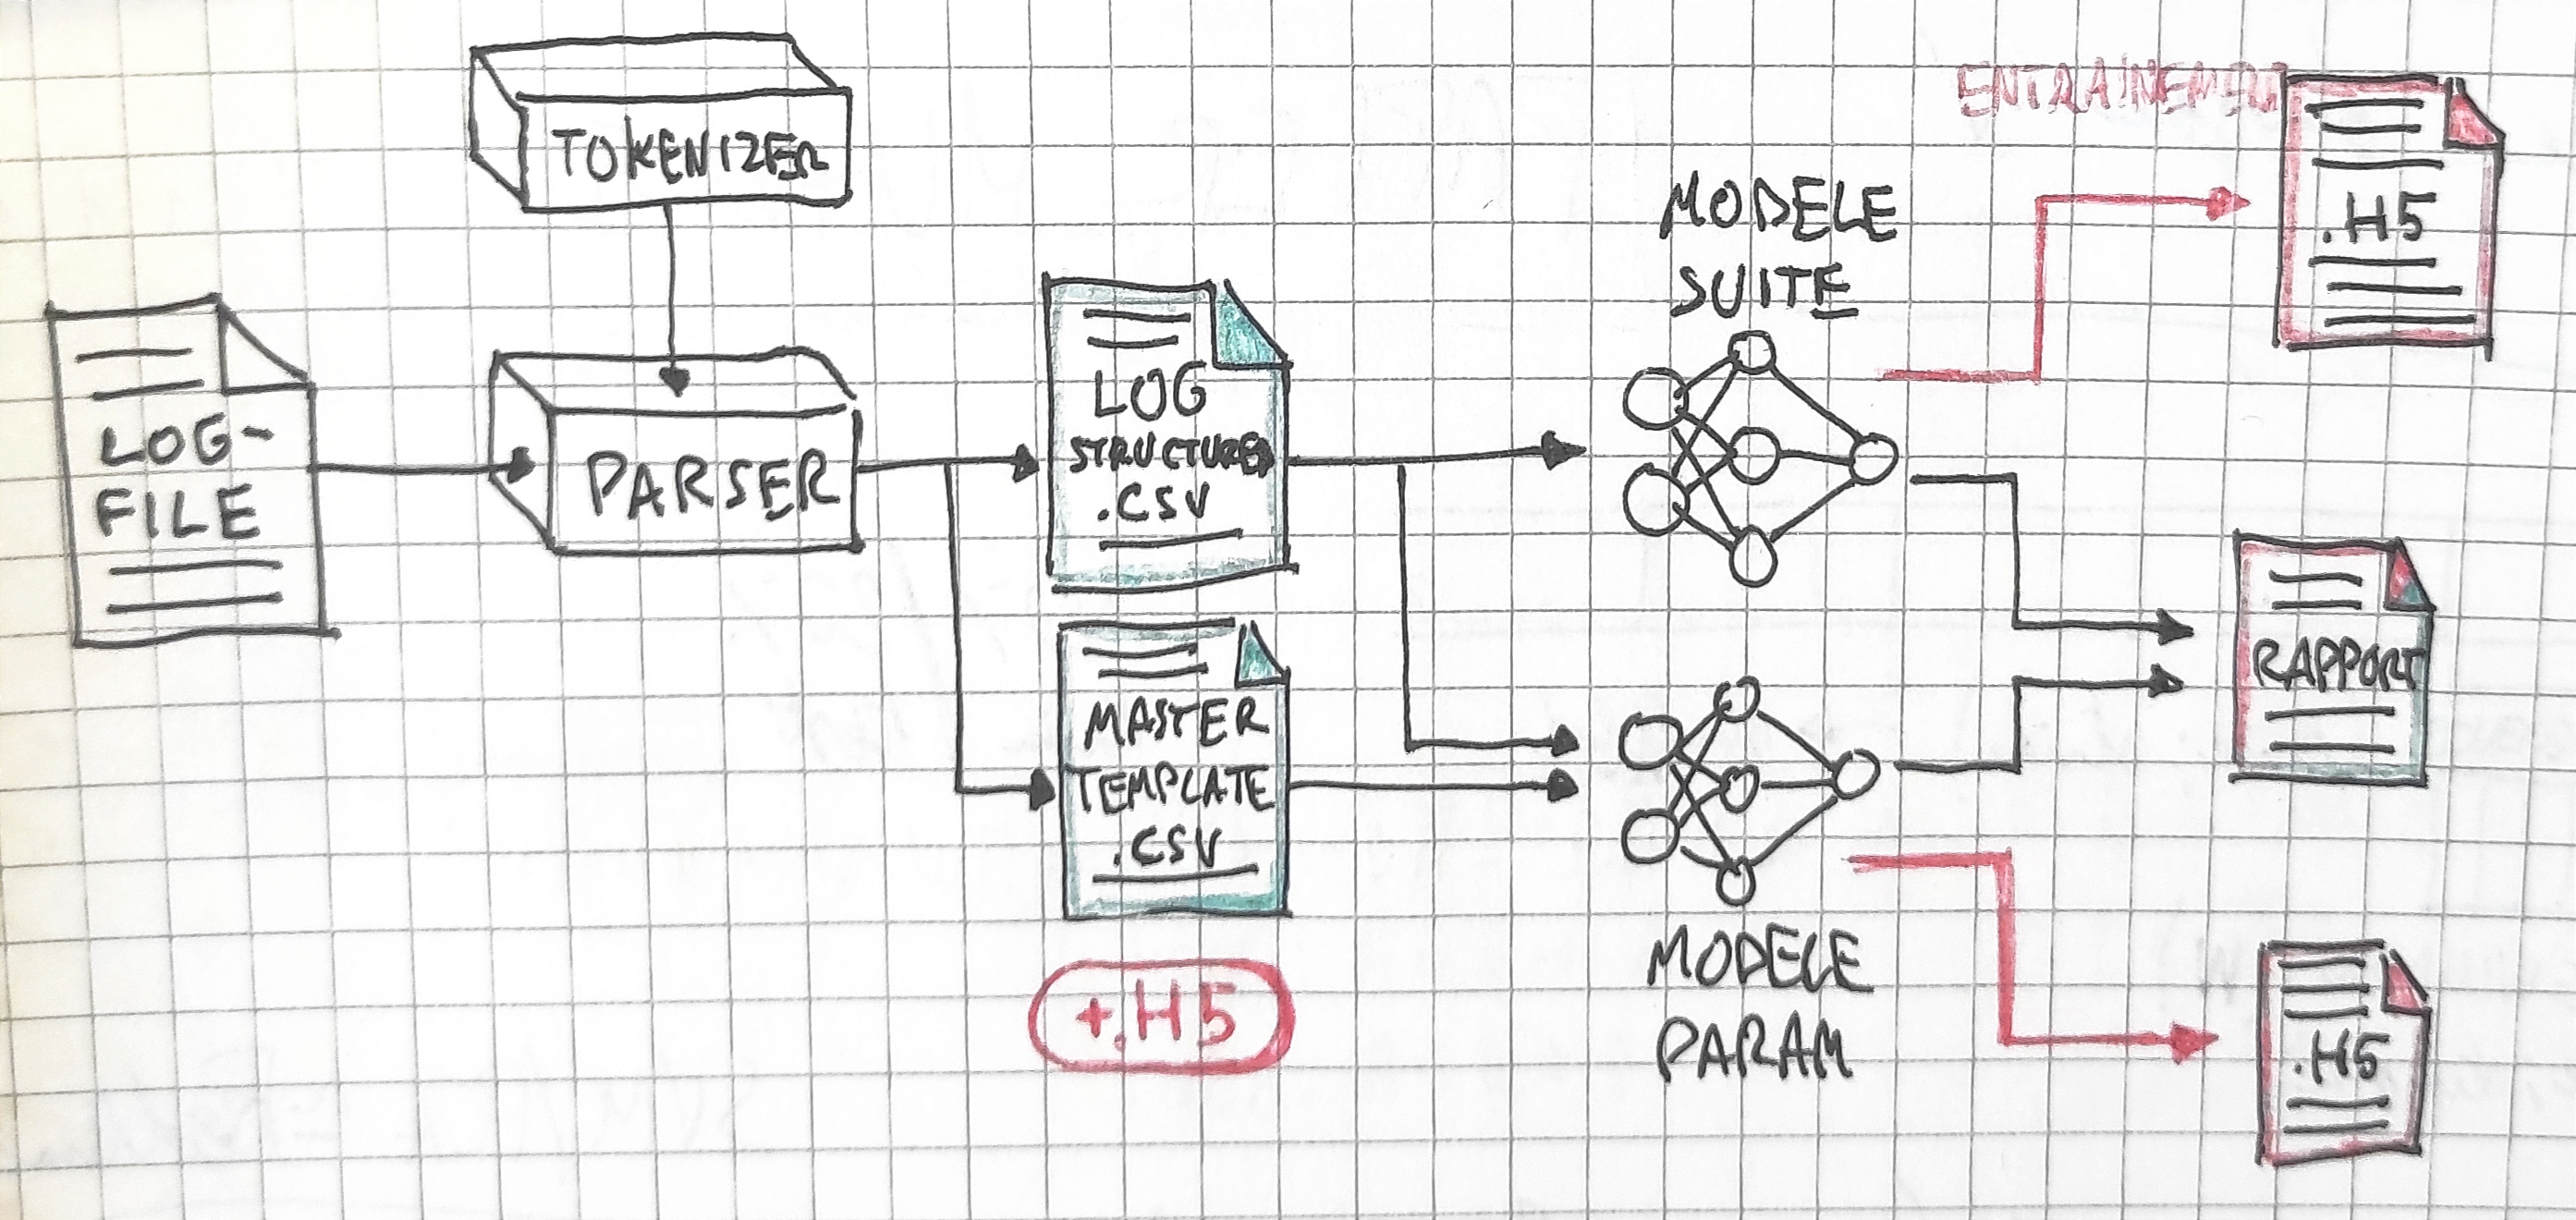
\includegraphics[width=0.6\textwidth]{images/analyselogs.jpg}
	\caption{Structure des modèles du projet original}
	\label{analyselogs}
\end{figure}

La figure \ref{analyselogs} décrit la structure des modèles d'analyse des \glspl{log} dans le projet original. Elle est très similaire à celle de DeepLog (voir figure \ref{deeplog}), étant donné que le projet a été à l'origine simplement une implémentation de cet algorithme. Un problème se pose quand on souhaite implémenter des algorithmes différents de DeepLog dans leur architecture. C'est d'ailleurs pour cette raison que Léa n'a pas implémenté d'autres algorithmes, mais simplement certains des blocs fonctionnels dans cette structure.

L'idée était donc de réécrire le projet, en partant non pas d'un algorithme en particulier mais d'une architecture permettant d'implémenter les différents algorithmes envisagés, et plus si nécessaire. Celle-ci devrait bien sûr inclure DeepLog, et donc la structure parseur $\rightarrow$ analyse suite / analyse paramètres doit être comprise dans l'architecture. En utilisant des structures de classes et d'héritage, beaucoup d'abstractions peuvent être faites.

\begin{figure}[ht]
	\centering
	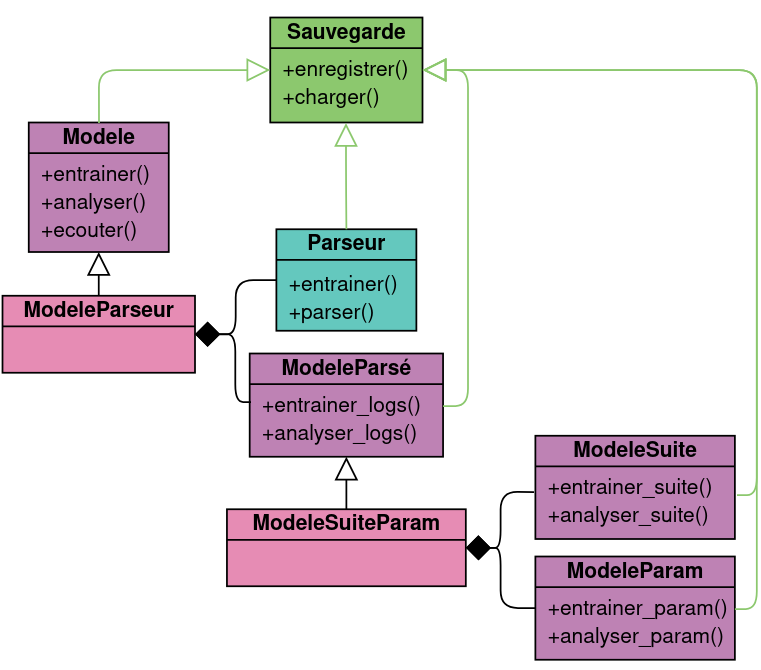
\includegraphics[width=0.6\textwidth]{images/archireecriture.png}
	\caption{Nouvelle architecture pour les modèles d'analyse}
	\label{archireecriture}
\end{figure}

La figure \ref{archireecriture} détaille la structure de classe pour les modèles de la réécriture. On peut voir beaucoup de similarités avec la structure précédente, mais celle-ci est déjà plus formalisée, et surtout il est envisageable d'y rajouter des composants. Cela est dû a la séparation des types de modèles, ainsi que leur abstraction. Un modèle complet est capable de s'entrainer, d'analyser un fichier de \glspl{log}, et d'écouter des \glspl{log} en direct. On n'a pas besoin de connaitre son fonctionnement interne si on l'utilise juste à haut niveau. Ce principe est utilisé a tous les niveaux de l'architecture, par exemple pour la sauvegarde: tous les types de modèles, ainsi que les parseurs, doivent pouvoir êtres enregistrés et chargés, et c'est donc défini par l'interface <<\texttt{Sauvegarde}>>.

\newpage
\chapter{Organisation du projet}

\section{La planification et les aléas}

Comme je l'ai mentionné plus haut, Robin a démarré son stage avant mon retour d'école. Il a donc fallu lui trouver des tâches à faire avant mon arrivée, afin d'utiliser efficacement tout le temps disponible pour le projet. Mon premier travail à donc été, avant la période d'école de Janvier, de faire une première planification des tâches, tout particulièrement sur la période de février.

Ce premier planning effectué est disponible en annexe \ref{planning}. Différents points sont intéressants à noter à son sujet. Tout d'abord, la possibilité d'un stage à l'étranger était toujours envisagée, mais suite à une absence de réponse de l'entreprise que j'avais contacté, j'ai décidé de suivre l'exercice de remplacement à la place. Cela a permis de libérer du temps pour la réalisation du projet, ce qui est intéressant vu le temps limité que j'aurais eu sinon.

J'aimerais aussi indiquer que les sprints définis dans ce planning étaient relativement libre dans leur contenu. L'idée principale était de développer, tester et comparer les algorithmes retenus pendant l'état de l'art tout en essayant de suivre un mode agile.

\bigskip
Notre méthode de travail avec Robin était très collaborative. Nous avons beaucoup discuté au fil du projet pour régler des problèmes, ou mieux comprendre des points particuliers. Nous avons eu très vite une bonne entente, et notre curiosité partagée vis à vis de la recherche et des sciences nous a permis de discuter de sujets très intéressants. Cette méthode collaborative est très intéressante dans le cadre d'un projet de recherche, car sa complexité était élevée, et nous n'aurions pas pu avancer aussi bien si on travaillait chacun de notre coté.

\bigskip
Le premier point qui va venir déranger le planning a été ma sous-estimation de la charge de travail liée à la partie académique du projet. En effet, la recherche peut être un processus lent et fastidieux. Dans le cadre de la méta-analyse (analyse de nombreux papiers de recherche pour en tirer des conclusions), ce n'est que plus vrai, nécessitant d'abord de trouver les bon papiers du domaine, puis de les comparer et en tirer des résultats.

Cet allongement des tâches de Robin m'a permis de commencer le développement de la réécriture du projet, qui n'était pas du tout prévue dans le planning à l'origine. Cette réécriture me prendra beaucoup de temps, et cela décalera encore le planning.

\bigskip
A la moitié du projet, un point à été fait pour regarder notre progression ainsi que l'évolution de la planification. Les changements de planning effectués sur la première moitié du projet, ainsi que les changements dans la planification future, sont reflétés dans le second planning en annexe \ref{planning2}. Les sprints ont été remplacés par des tâches précises, nous avons donc abandonné l'agilité. Je vais donc détailler les obstacles à l'utilisation des méthodes agiles, ainsi que les causes dans notre projet, dans la partie suivante.

\section{Les freins à l'agilité}

L'agilité est une approche à la gestion de projet née du manifeste agile, basée sur 4 valeurs simples: (<<{>}>> représente <<plutôt que>>)

\begin{itemize}
	\item Individus et interactions > Processus et outils
	\item Logiciel fonctionnel > Documentation exhaustive
	\item Collaboration avec le client > Négociation contractuelle
	\item Adaptation au changement > Exécution d'un plan
\end{itemize}

De ces points naissent différentes méthodes telles que Scrum, qui décrit un cadre plus précis sur la mise en place et la réalisation de cette gestion de projet. Des <<sprints>> sont mis en place, qui séparent le temps du projet en cycles courts itératifs (en moyenne autour de quelques semaines). A chaque sprint, différentes tâches sont attribuées aux développeurs, et une démonstration de ce qui a été réalisé est faite à la fin.

\bigskip
Les méthodes agiles s'appliquent très bien au développement informatique, et c'est majoritairement dans ce domaine qu'elles sont utilisées. Mais une étude publiée en 2013 \cite{obstacles} met en avant les différents facteurs qui peuvent freiner leur mise en place, et nous allons les détailler dans cette partie. Le papier met en avant le fait que ces freins à l'agilité sont en majorité causés par la culture et la structure trop traditionnelle des organisations concernées.

Les managers/chefs de projets sont aujourd'hui au centre du fonctionnement des méthodes industrielles de développement logiciel. La structure typique des grandes organisations est celle d'une hiérarchie a de nombreux niveaux, définissant des structures de commande et de prise de décision. Dans les méthodes agiles, le rôle du manager devient celui de leader. Il devient un facilitateur de la collaboration au sein de l'équipe, ainsi que de la créativité de ses membres. De plus, la structure de décision est en partie retournée, les développeurs étant source d'idées et de propositions que le manager se doit de remonter dans la hiérarchie. Ce premier point peut être un des plus difficiles, nécessitant une compréhension par le manager du changement de son positionnement dans le cycle de développement. Il ne faut pas qu'il garde une position de commande et de contrôle sur les membres de l'équipe, qui serait contre productive.

Cela nous mène à parler du coût de ce changement, plus précisément le coût de la formation des différents acteurs. En effet, si les managers doivent être préparés à ce changement drastique de leur positionnement par des formations, ils ne sont pas les seuls à devoir modifier leur mode de travail. Les développeurs deviennent plus responsabilisés, à la fois au sein de la structure et du projet. La collaboration n'est pas toujours évidente, notamment dans le cas de méthodes comme le <<pair programming>> qui pourraient en déstabiliser certains. Le dernier acteur qu'il faut former, peut être le plus important mais le plus difficile, est le client. Sa place est centrale dans toute méthode agile, car il doit être capable de faire des retours rapide à l'équipe pour permettre le développement continu du produit. Simplement trouver le bon interlocuteur pour cette tâche peut être très compliqué, car il doit avoir des responsabilité et de la connaissance tout en restant disponible et collaboratif.

Un autre point qui va à l'encontre des méthodes traditionnelles est la petite quantité de planification et de documentation produite dans le cycle de développement. Une méthode industrielle classique telle qu'une cascade \cite{waterfall} ou un cycle en V se base fortement sur une planification complète du projet a priori, et tout le développement suivant doit se caler sur ce planning. Il peut être difficile pour une organisation de se passer de l'étape de planification, ou du moins de la limiter a un planning très général et vague, étant donné le temps et l'importance qu'elle a dans une méthode traditionnelle. La documentation est elle aussi un point de contention, étant elle aussi gardée au minimum dans les méthodes agiles. Dans une méthode traditionnelle, la documentation fait partie du développement au même titre que les tests, permettant de valider l'existence de la fonctionnalité. Encore une fois, il pourrait être difficile pour une équipe qui y est habituée de s'en passer.

Enfin, le choix des outils et méthodes n'est pas toujours évident pour une équipe nouvelle à l'agilité. Il existe de nombreuses méthodologies fondées sur les principes agiles (XP, Scrum, TDD...) et il n'est pas facile de savoir lesquelles correspondront à une équipe et un projet donné. De plus, des nouveaux outils devront être mis en place pour répondre a des nouveaux besoins (intégration continue, gestion de version, qualité de code) qui n'étaient pas nécessairement présents ou adaptés, et beaucoup de différents outils existent pour résoudre un ou plusieurs de ces problèmes. Le coût en terme de temps pour trouver des solutions qui nous conviennent est donc élevé.

\bigskip
Certains des points mentionnés ici s'appliquent en effet à notre situation, mais des nuances sont présentes dans le contexte d'un projet de recherche. Nous étions aussi un binôme, et nous n'avions pas de méthodologies précédentes pour nous faire former des aprioris.

Le temps de formation était un de nos plus gros problème. Si j'ai effectivement étudié les méthodes agiles en cours, je n'ai jamais réellement eu l'occasion de les mettre en pratique dans mes projets. L'utilisation assez limitée de l'agilité dans les projets de la \gls{DGFiP}, ainsi que mon manque d'implication dans d'autres projets, ont limité mon expérience de terrain avec ces méthodes, et il était donc difficile pour moi de les mettre en place. C'est un point que je trouve dommage, et j'aurais dû y faire plus attention, car un projet de recherche se porte en réalité très bien à l'utilisation de l'agilité. En effet, le fait de partir d'une problématique relativement vague, et d'incrémentalement améliorer les objectifs ainsi que le projet est exactement le but de l'agilité. Il est intéressant de noter qu'il existe des façons d'appliquer les méthodes agiles avec un seul développeur \cite{agilesolo} \cite{ssdm}.

\newpage
\chapter{Projection de l'impact du projet}

\section{Gain de temps et de productivité}

\todo{Partie éco}

\section{L'humain contre la machine}

L'intelligence artificielle est une technologie qui a connu une grande expansion durant cette décennie, et comme toute technologie, a connu des éloges ainsi que des critiques. Mais plus elle est présente dans notre vie, plus les peurs liées à son utilisation se font ressentir. En grande partie, les gens ont peur d'une chose: la perte de leur travail aux dépens d'une machine. Nous allons étudier cette thèse avec l'aide d'un chapitre du livre <<Le futur du travail>> \cite{futurtravail} par J.S. Carbonell, chercheur en sciences sociales du travail.

Dans ce chapitre, Carbonell met en avant le fait que le travail n'est pas simplifié (et ne disparaît pas) par l'automatisation, bien au contraire. Les machines ne nous remplacent pas autant qu'elles changent notre relation au travail, mis en évidence par le fait que malgré ce mouvement d'automatisation, il n'y a pas de rupture du marché du travail pour cette raison. En effet, derrière l'automatisation se cachent de nombreux métiers que Carbonell appelle <<invisibles>>, le revers de la médaille étant la précarité de ces travailleurs de l'ombre.

En fonction des industries, les effets et les mécanismes de l'automatisation sont vastes et variés, et le remplacement du travail n'en est qu'une unique facette. Dans la suite de cette partie, nous allons détailler les conséquences que l'automatisation peut apporter au travail, telles que décrites par Carbonell.

\bigskip
La première, mais surtout la plus <<fantasmée>>, est le remplacement du travail humain par le travail d'une machine. L'exemple ici est donné de l'atelier de peinture d'une chaîne de production automobile: <<Un robot peut enregistrer toutes les 20 millisecondes la position d'un ouvrier peintre, ce robot est ensuite capable de reproduire exactement la séquence de l'opération qui à été enregistrée et, ainsi, de confisquer des séquences entières du travail ouvrier.>> Le remplacement est d'autant plus facile que le travail est répétitif, l'exemple des lignes de production d'usine est donc tout particulièrement pertinent. On pourra mentionner <<Les temps modernes>> de Charlie Chaplin, qui critique de manière humoristique le remplacement des ouvriers dans ces usines de production.

Carbonell explique la cause de l'attention portée a cette conséquence à l'industrie sidérurgique, pour laquelle un levier de réduction de la masse salariale était l'automatisation de substitution. Elle apportait un très grand gain de temps et de moyens aux industries, avec des suppressions de jusqu'à deux tiers des effectifs.

\bigskip
La seconde conséquence est décrite comme un processus de <<déqualification/requalification>> du travail. La suppression de tâche ne pousse pas forcément à la suppression de postes, et il est possible de redistribuer le travail restant parmi les employés. Selon les observations de Carbonell, cela provoque un mouvement symétrique où <<une partie de la main d'œuvre est déqualifiée ou déclassée, une autre est requalifiée ou reclassée.>>

La déqualification est facile à expliquer: La division du travail crée des tâches faciles à automatiser, et ce qui reste pour les employés est du travail le plus simple et sans intérêt possible. L'économiste Benjamin Coriat, cité par Carbonell, parle de <<taylorisation assistée par ordinateur>>.

La requalification est provoquée par la nature même de l'automatisation, à travers la maintenance, la programmation, ou même la surveillance des machines. Cela peut avoir des effets positifs, par exemple des ouvriers de production qui deviennent des ouvriers d'entretien, mais aussi des effets négatifs, tels que le licenciement des salariés moins qualifiés. En effet, le coût de formation pour la requalification d'un employé n'est pas négligeable, et il peut être parfois plus intéressant d'embaucher de nouveaux travailleurs déjà qualifiés. Il est aussi possible que de requalifier certains puisse déqualifier d'autres, revenant a l'effet symétrique mentionné plus haut.

\bigskip
La troisième conséquence de l'automatisation est appelée <<intensification>> du travail. Carbonell décrit par ce mot différents facteurs: <<l'augmentation des rythmes de travail, la dégradation de la santé et de la sécurité au travail, la hausse de la charge physique [et mentale]>>. Il explique ce point par les motivations des employeurs à l'automatisation: si on automatise les taches simples et répétitives, les salariés se retrouvent avec les tâches qui apportent plus de valeur pour l'entreprise, et qui demandent donc plus de travail. On optimise non pas seulement les tâches qui sont automatisées, mais aussi celles qui ne le sont pas, sur lesquelles les employés vont pouvoir se concentrer.

\bigskip
La quatrième et dernière conséquence est le contrôle, ou l'augmentation du pouvoir de la direction sur les salariés. Il est possible, à travers les machines et l'informatique, de surveiller les temps de travail, les périodes de pauses, la productivité des employés... De plus, certaines de ces technologies sont mises en place spécifiquement dans le but de contrôler ou surveiller le lieu de travail.

\newpage
\chapters{Conclusion}

\stoplist[main]{lof}

% BIBLIOGRAPHIE
\newpage
\backmatter
\pagenumbering{gobble}
\pagestyle{plain}

\bibliography{biblio}

% GLOSSAIRES
\printglossary[type=admin,nonumberlist]
\newpage
\printglossary[type=tech,nonumberlist]

% FIGURES
\newpage
\printlist[main]{lof}{}{\chapters{Table des figures}}


% ANNEXES
\newpage
\appendix

\startlist[appendix]{lof}
\printlist[appendix]{lof}{}{\chapters{Annexes}}
\newpage

\anneximage{orga}{90}{Organigramme des services de la \gls{DGFiP}}
\anneximage{orga_si}{0}{Organigramme des bureaux du \gls{SI}}
\anneximage{planning}{90}{Planning original du projet}
\anneximage{planning2}{90}{Planning mis à jour au milieu du projet}

\listoftodos

\end{document}
